\documentclass[tikz,border=5pt]{standalone}
\usepackage{amssymb,amsmath}
\newcommand{\C}{\mathbb{C}}
\newcommand{\CP}{\mathbb{CP}}
\begin{document}
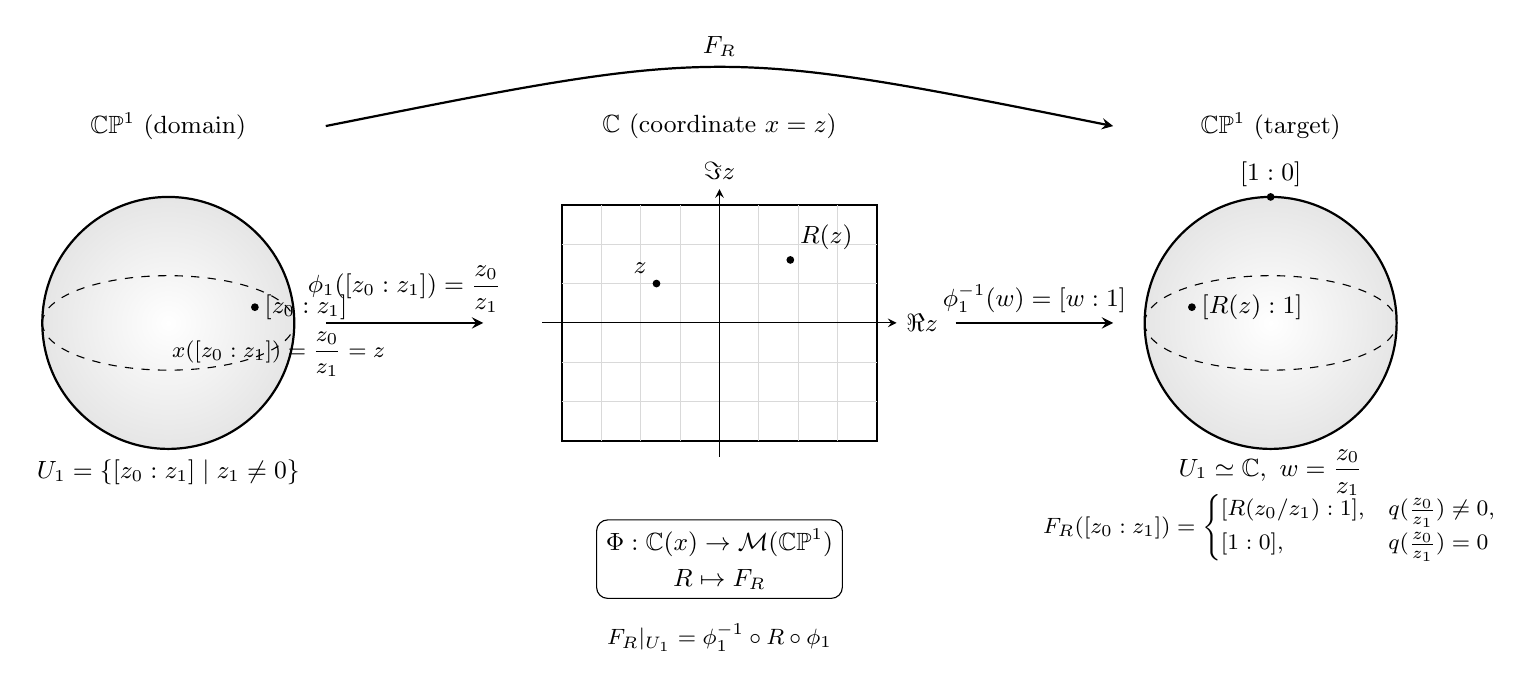
\begin{tikzpicture}[font=\small,>=stealth]
%\draw[gray!50, dashed] (-5,-5) grid (5,5);	
%\foreach \i in {-4,...,-2,-1,1,2,...,4}
%\draw[] (\i,.1)--(\i,-.1) node[below] {$\i$};%x-axis
%\foreach \i in {-4,...,-2,-1,1,2,...,4}
%\draw[] (.1,\i)--(-.1,\i) node[left] {$\i$};%y-axis
	
%========================================
% LEFT: Domain CP^1 with affine chart U_1
%========================================
\begin{scope}[shift={(-7,0)}]
	% Sphere = CP^1 (domain)
	\shade[inner color=white, outer color=gray!20, draw=black, thick]
	(0,0) circle (1.6);
	\node at (0,2.5) {$\CP^1$ (domain)};
	
	% Equator = U_1
	\draw[dashed] (-1.6,0) arc (180:360:1.6 and 0.6);
	\draw[dashed] (-1.6,0) arc (180:0:1.6 and 0.6);
	\node at (0,-1.9) {$U_1=\{[z_0:z_1]\mid z_1\neq 0\}$};
	
	% Point [z0:z1] in U_1
	\fill (1.1,0.2) circle (1.4pt);
	\node[right] at (1.1,0.2) {$[z_0:z_1]$};
	\node at (1.4,-0.4) {\footnotesize $x([z_0:z_1])=\dfrac{z_0}{z_1}=z$};
\end{scope}
%========================================
% MIDDLE: Complex plane C (affine coord)
%========================================
\begin{scope}[]
% Rectangular region for C
\draw[thick] (-2,-1.5) rectangle (2,1.5);
\node at (0,2.5) {$\C$ (coordinate $x=z$)};

% Grid
\foreach \x in {-1.5,-1,...,1.5}
\draw[gray!30] (\x,-1.5) -- (\x,1.5);
\foreach \y in {-1,-0.5,...,1}
\draw[gray!30] (-2,\y) -- (2,\y);

% Axes
\draw[->] (-2.25,0) -- (2.25,0) node[right] {$\Re z$};
\draw[->] (0,-1.7) -- (0,1.7) node[above] {$\Im z$};

% Point z and its image R(z)
\fill (-0.8,0.5) circle (1.4pt);
\node[above left] at (-0.8,0.5) {$z$};

\fill (0.9,0.8) circle (1.4pt);
\node[above right] at (0.9,0.8) {$R(z)$};

%% Arrow z -> R(z)
%\draw[->,thick]
%(-0.8,0.5) .. controls (-0.2,1.2) .. (0.9,0.8);
%\node at (0.0,1.4) {$R(x)=\dfrac{p(x)}{q(x)}\in\C(x)$};

%% Indicate a zero of q (pole of R)
%\fill (1.6,0.0) circle (1.4pt);
%\node[below] at (1.6,0.0) {\footnotesize $q(z)=0$};
%\draw[->,densely dashed] (1.6,0.0) -- (2.1,-0.8);
%\node at (2.4,-1.0) {\footnotesize ``$\infty$''};
\end{scope}
%========================================
% RIGHT: Target CP^1 with image F_R
%========================================
\begin{scope}[shift={(7,0)}]
	% Sphere = CP^1 (target)
	\shade[inner color=white, outer color=gray!20, draw=black, thick]
	(0,0) circle (1.6);
	\node at (0,2.5) {$\CP^1$ (target)};
	
	% Equator (affine chart U_1 of target)
	\draw[dashed] (-1.6,0) arc (180:360:1.6 and 0.6);
	\draw[dashed] (-1.6,0) arc (180:0:1.6 and 0.6);
	\node at (0,-1.9) {$U_1\simeq\C,\ w=\dfrac{z_0}{z_1}$};
	
	% North pole = [1:0]
	\fill (0,1.6) circle (1.4pt);
	\node[above] at (0,1.6) {$[1:0]$};
	
	% Image of non-pole: [R(z):1]
	\fill (-1,0.2) circle (1.4pt)
	node[right] {$[R(z):1]$};

	% Caption for definition of F_R
	\node at (0,-2.6) {\footnotesize $F_R([z_0:z_1])=
		\begin{cases}
			[R(z_0/z_1):1], & q(\tfrac{z_0}{z_1})\neq 0,\\
			[1:0], & q(\tfrac{z_0}{z_1})=0
		\end{cases}$};
\end{scope}
%========================================
% ARROWS: charts and composition F_R
%========================================

% Chart phi_1: CP^1 (domain) -> C
\draw[->,thick]
(-5,0) -- (-3,0)
node[midway, above] {$\phi_1([z_0:z_1])=\dfrac{z_0}{z_1}$};

% Chart phi_1^{-1}: C -> CP^1 (target)
\draw[->,thick]
(3,0) -- (5,0)
node[midway, above] {$\phi_1^{-1}(w)=[w:1]$};

% Big arrow: F_R: CP^1 -> CP^1
\draw[->,thick]
(-5,2.5) .. controls (0,3.5) .. (5,2.5)
node[midway, above] {$F_R$};

% Label for the commutative picture
\node at (0,-4) {\footnotesize $F_R|_{U_1}=\phi_1^{-1}\circ R\circ\phi_1$};
% Label for Φ: C(x) -> M(CP^1)
\node[draw,rounded corners,align=center] at (0,-3)
{$\Phi:\C(x)\to\mathcal{M}(\CP^1)$\\[2pt]
	$R \mapsto F_R$};
\end{tikzpicture}
\end{document}